\subsection{Retrieving single source position in free field}

The purpose of this experiment is to test the sound localization algorithms in a controlled environment. A tetrahedral array receives sound waves emitted by a point source and its location is  retrieved. The point source position is fixed and the microphone array is rotated around its axis in order to change the receiving angle of the wave. A diagram of the setup is display in figure \ref{fig:Anechoic1} where the two point source position are shown: 90 and 30 degree.  The source is chosen to be a pink noise as in our simulation but recording of a 300Hz sinusoid are performed to check the delay between the microphones. In order to recreate the far field condition in the limited space of the anechoic chamber the array is placed as further away from the source and the array aperture is reduced in order to reduce the size of the array and obtain a better plane wave propagation. 

\begin{figure}[H]
    \centering
    \includegraphics[width=0.7\textwidth]{Figures/Anechoicexp1.png}
    \caption{Diagram of the experiment}
    \label{fig:Anechoic1}
\end{figure}
 

\subsubsection{Stimuli and settings}

The point source is created by a Brüel \& Kjær omnisource type 4296 with operating frequency of 100 to 5000 Hz. The Brüel \& Kjær PULSE system is used to record the sound picked up by the microphone array and the operating frequency of the system is 131072 Hz which is the highest sampling frequency available on the system. Algorithm parameters are temperature: 22 $\degree$ and speed of wind: 0 m/s. The prototype microphone array allows to adjust the aperture size from 0,1m to 1m. As discussed earlier the aperture is reduced to 0,395m. When strong periodicity in the signal, the array can in theory work with waves of frequency up to 874 Hz before aliasing occurs. In our case there is no strong periodicity when we are using pink noise as sound sources, much higher frequencies can be input \ref{REF}.

\begin{equation}
    f=\frac{c}{\lambda}=\frac{345}{0,395} \approx 874 (Hz)
\end{equation}

 
\subsubsection{Delay between the microphones}
 
 In order to know the accuracy of the measurements, sample delay is measured at a single frequency. In order to avoid the pressure field frequency zone of the anechoic chamber and array aliasing,  a sin wave of 300 Hz is choosen. A single frequency is chosen to avoid group delay issues.  
 
 \begin{figure}[H]
    \centering
    \includegraphics[width=0.8\textwidth]{Figures/delaytetra300Hz.png}
    \caption{sin wave recorded by the four microphones.}
    \label{fig:pinknoise}
\end{figure}
 
 
\begin{center}
  \begin{tabular}{ | l | c | r | r | r |}
    \hline
    Delays & Mic 1 & Mic 2 & Mic 3 & Mic 4 \\ \hline
    Mic 1 & X & -6&114 & 52  \\ \hline
    Mic 2 &   & X &120 & 58  \\ \hline
    Mic 3 &   &   & X  &-61  \\ \hline
    Mic 4 &   &   &    & X   \\ \hline
  \end{tabular}
  \captionof{table}{Sample delay measured between the microphones at 0 incidence (Fs= 131072Hz)}
\end{center}

Variation in delay are due to the source position inaccuracies or could be due to the plane wave approximation not holding. Therefore wider peaks are to be expected and a slight shift from the zero degree position. The microphones are not calibrated in this experiment as we can see difference in amplitude are noticeable.
 
\subsubsection{Results}

Wave files recorded by the pulse system are used by the algorithm. The script "NAMEOFTHESCRIPT" is run and the energy maps of the SRP-PHAT and minimum power SRP-PHAT algorithms are computed and displayed in the following part.


\begin{figure}[H]
    \centering
    \begin{subfigure}[b]{0.96\textwidth}
    \centering
    \includegraphics[width=0.95\textwidth]{Figures/Anechoic0Deg1SrcNorm.png}
\end{subfigure}
\vskip \baselineskip
\begin{subfigure}[b]{0.96\textwidth}
    \centering
    \includegraphics[width=0.95\textwidth]{Figures/Anechoic0Deg1SrcMinPow.png}
\end{subfigure}
\caption{Figures depict from top-to-bottom SRP-PHAT and minimum power SRP-PHAT localization for source around (90 $\degree$, 0$\degree$) in the Anechoic Room}
\end{figure}

The source position is not exactly spot on at 90 degree azimuth incidence also we observe a slight elevation of the source. This is explained by the top microphone being on the same horizontal axis as the acoustic center of the sound source thus creating a slight shift up. 
%This shift can also be explained by the inaccuracies in the microphone positions on the microphone array. The prototype microphone array allows the 3 microphones on the horizontal axis to move up and down in order to adjust the microphone array aperture relative to the "fixed" top microphone. Therefore there might be a maladjustment in the position of the 3 lower microphones relative to the top microphone thus creating an incorrect position on the vertical axis and ultimately an error in the localization. 
The height of the microphone array is later increase in order to place the 3 lower microphones on the same vertical axis as the acoustic center of the sound source. The following figure shows the results for source at (30 $\degree$, 0$\degree$)
%As will be seen in the following graphs of the sound source at 30 $\degree$ azimuth the elevation error is reduced. No further investigation are done. 

\begin{figure}[H]
    \centering
    \begin{subfigure}[b]{0.96\textwidth}
    \centering
    \includegraphics[width=0.95\textwidth]{Figures/Anechoic30Deg1SrcNorm.png}
\end{subfigure}
\vskip \baselineskip
\begin{subfigure}[b]{0.96\textwidth}
    \centering
    \includegraphics[width=0.95\textwidth]{Figures/Anechoic30Deg1SrcMinPow.png}
\end{subfigure}
\caption{Figures depict from top-to-bottom SRP-PHAT and minimum power SRP-PHAT localization for source at 30 degree}
\end{figure}

\newpage
\subsection{Retrieving the multi-sources location and relative level in free field}

Another experiment is setup in the anechoic chamber with focus on retrieving the relative source levels difference of two sources playing at the same time. One source is placed at (90 $\degree$, 0$\degree$) and plays a pink noise at 46dBA, the second source is placed at (130 $\degree$, 0$\degree$) and plays an uncorrelated pink noise at 52dbA. The files are generated in matlab and low frequencies are filtered out in order to accommodate for the speaker used. Two custom spherical speakers are used to play the source signal and the aperture size of the array is 0.395m. Temperature of the room is 22 $\degree$ and wind is 0 m/s.

\begin{figure}[H]
    \centering
    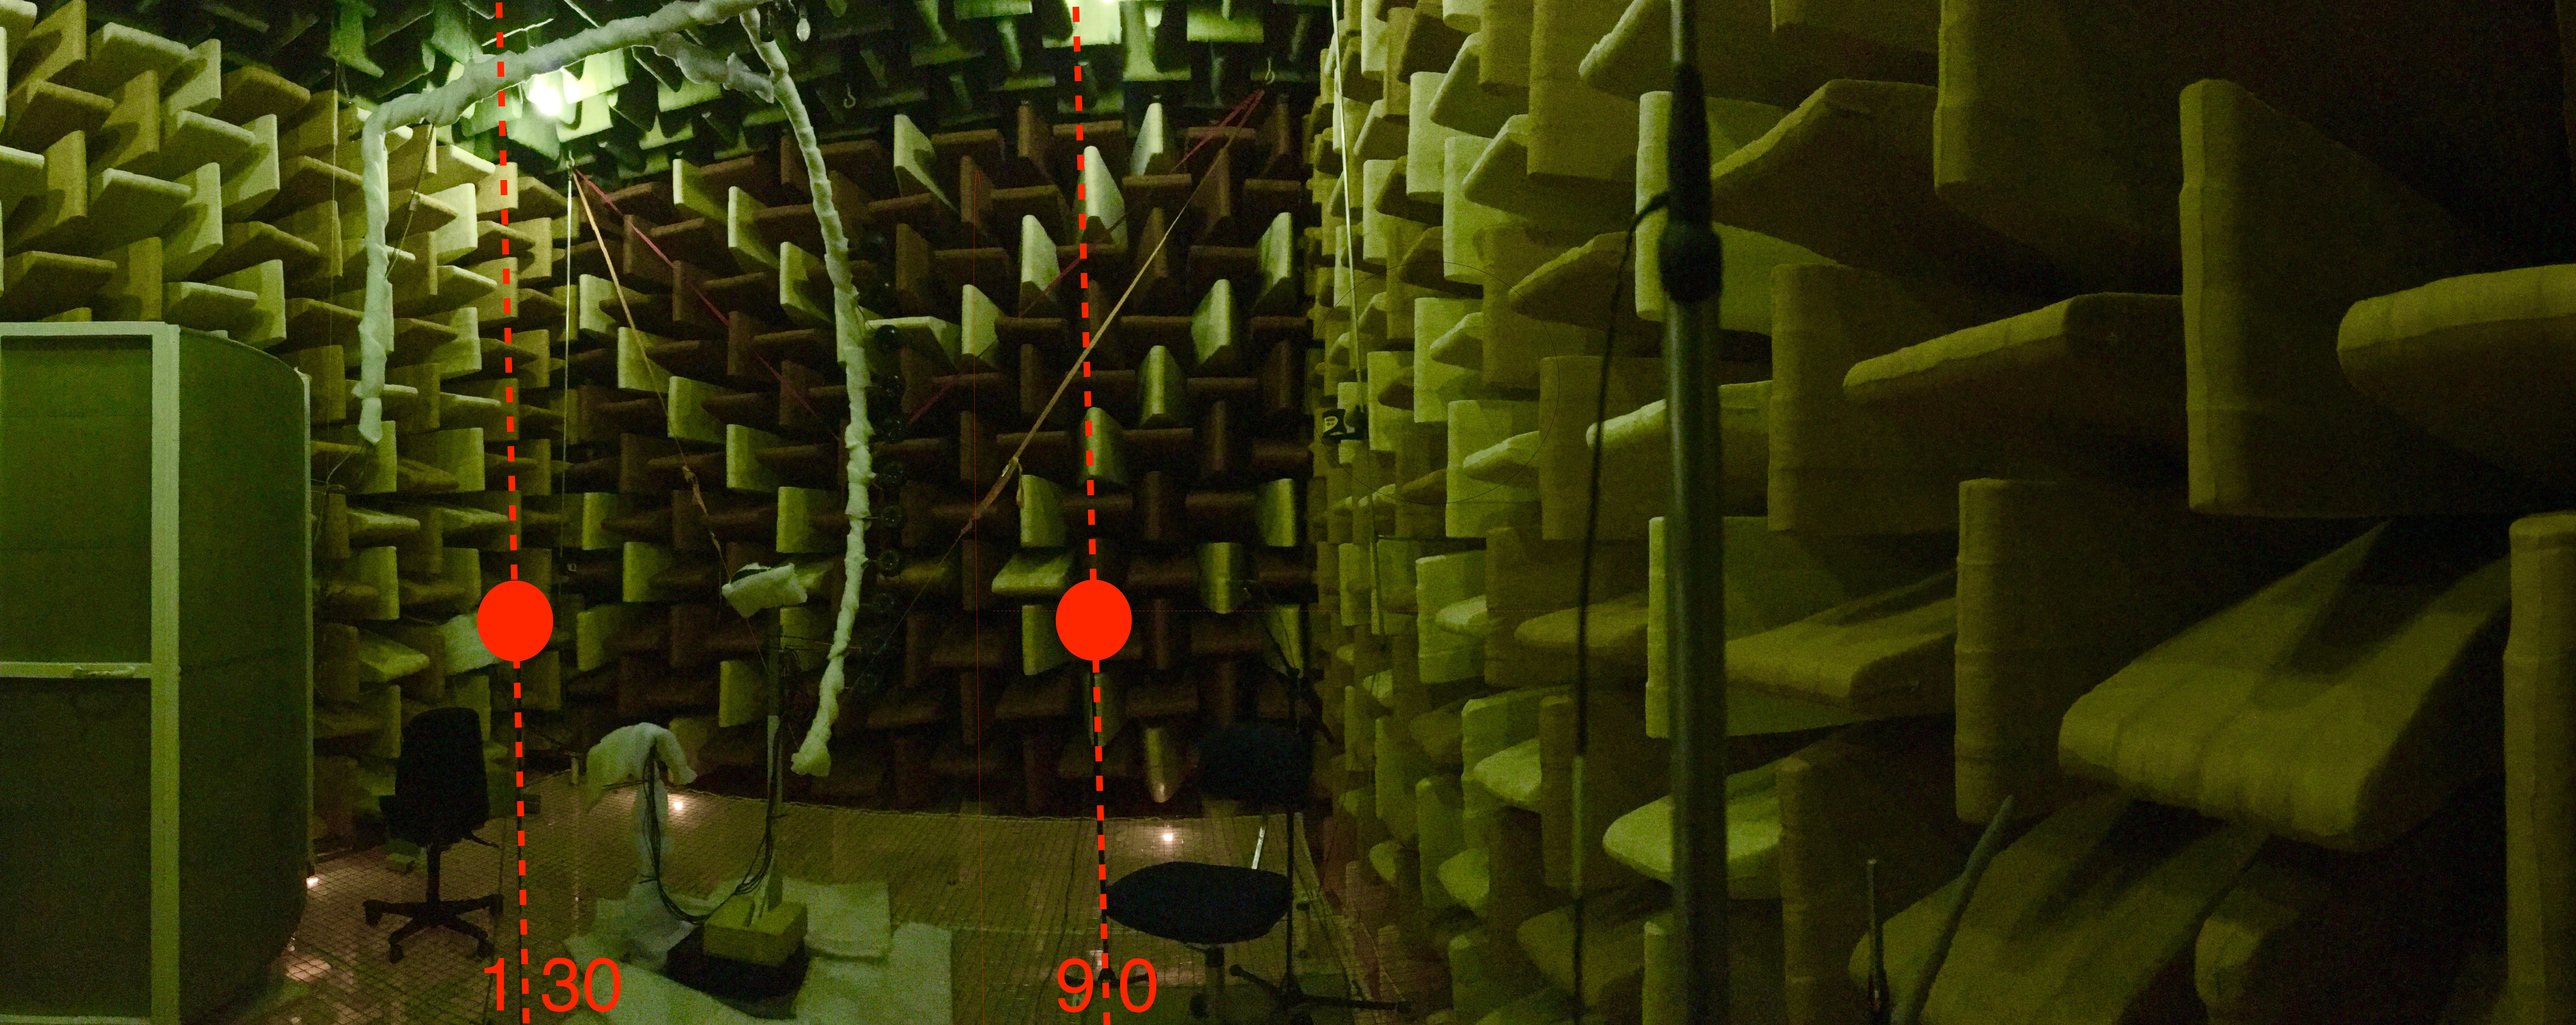
\includegraphics[width=1\textwidth]{Figures/AnechoicPic.jpg}
    \caption{Picture of the set up. The anechoic chamber was filled with misc. equipment, therefore the sources have been replaced by red dots for clarity. 90 and 130 $\degree$ azimuth are also drawn on top of the picture.}
    \label{fig:Anechoicpic1}
\end{figure}

\begin{figure}[H]
    \centering
    \includegraphics[width=0.7\textwidth]{Figures/Anechoicexp3.png}
    \caption{Diagram of the experiment}
    \label{fig:Anechoicexp3}
\end{figure}

\subsubsection{Results}

\begin{figure}[H]
    \centering
    \begin{subfigure}[b]{0.96\textwidth}
    \centering
    \includegraphics[width=0.95\textwidth]{Figures/Anechoic2SrcNorm.png}
\end{subfigure}
\vskip \baselineskip
\begin{subfigure}[b]{0.96\textwidth}
    \centering
    \includegraphics[width=0.95\textwidth]{Figures/Anechoic2SrcMinPow.png}
\end{subfigure}
\caption{Figures depict from top-to-bottom SRP-PHAT and minimum power SRP-PHAT localization}
\end{figure}


%
%\begin{figure}[H]
%    \centering
%    \begin{subfigure}[t]{0.5\textwidth}
%    \centering
%    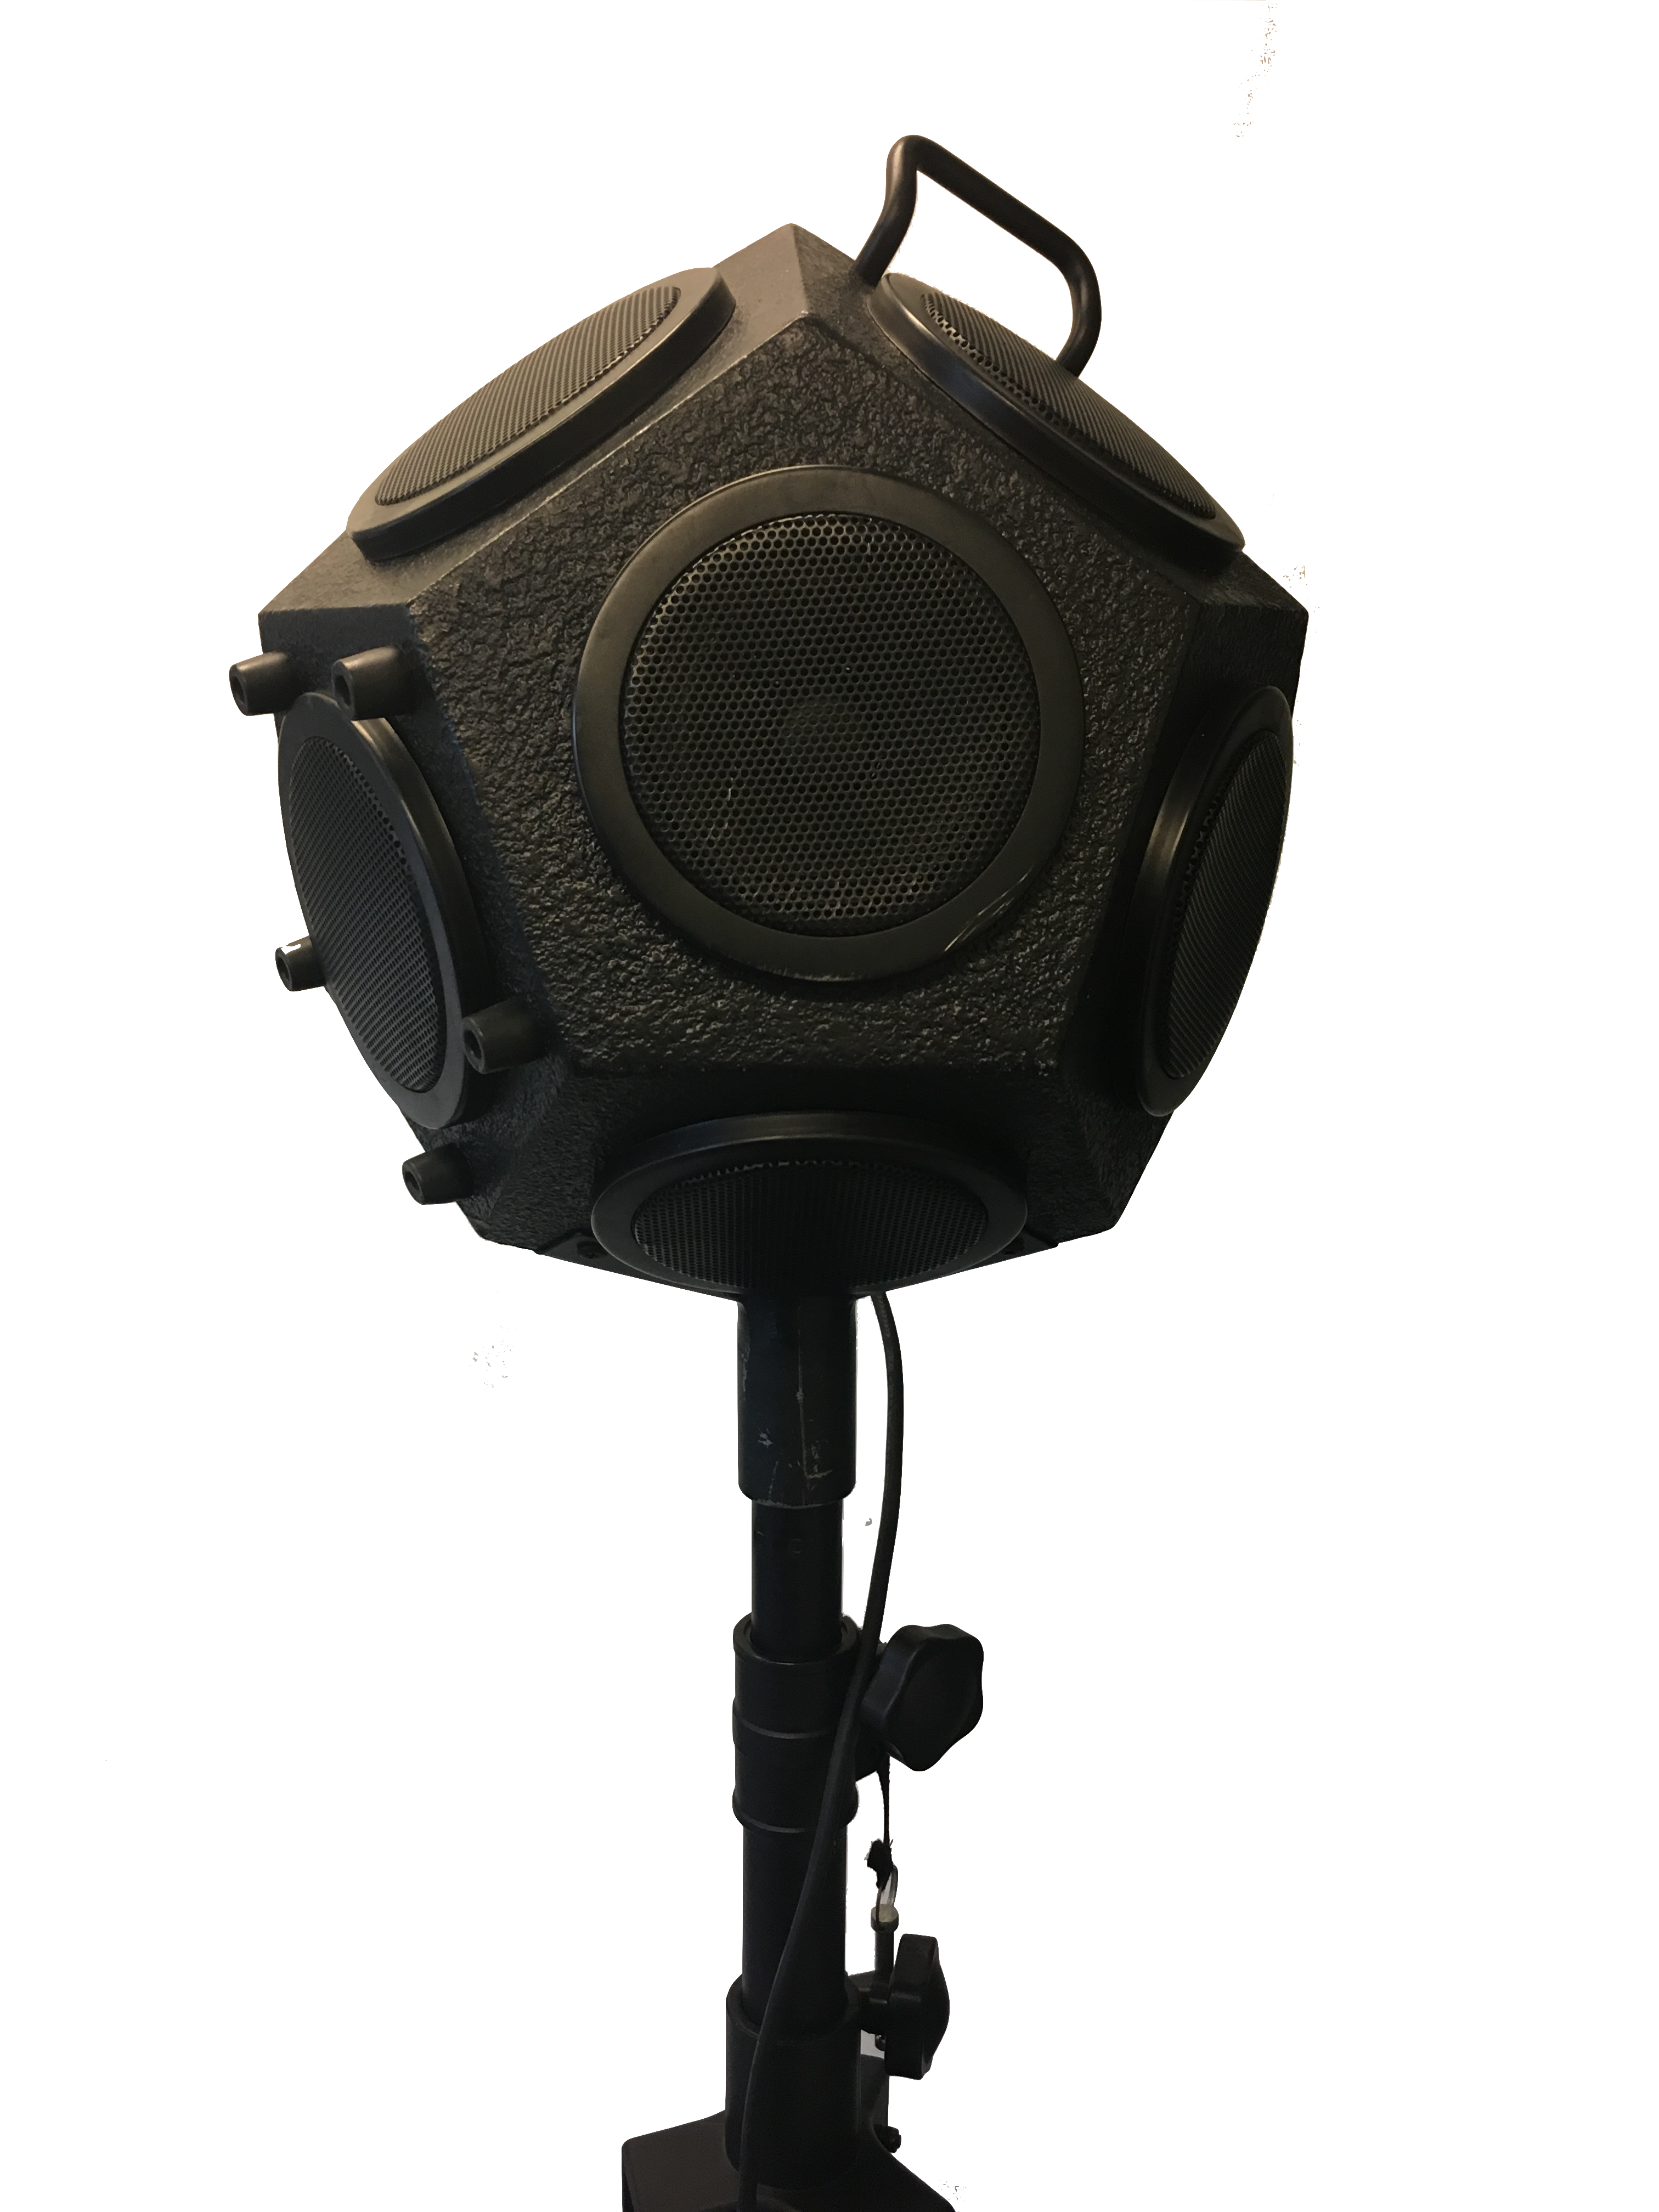
\includegraphics[width=0.9\textwidth]{Figures/IMG_7337.png}
%    \caption{B\&K Omnisource}
%    \label{fig:Omnisource}
%\end{subfigure}%
%\begin{subfigure}[t]{0.5\textwidth}
%        \centering
%    \includegraphics[width=0.9\textwidth]{Figures/Arraymicrophone.png}
%    \caption{Prototyped microphone array}
%    \label{fig:Array}
%\end{subfigure}
%\end{figure} 


\newpage
\subsection{One static source on a construction field}

In order to test the algorithm in a real conditions, several measurements are made on a construction field. Rather than using artificial source placed in the field at a known azimuth and elevation, real sources are used. In the first scenario one construction machine has a fixed position and produces noise that is recorded by the microphone array. Pictures are taken using a camera with a known focal length in order to retrieve the source azimuth. The aperture of the microphone array is 1 meter and the sources are more than 30 meters away. The measurement system is setup in the middle of the road in order to avoid too much pressure buildup near the wall boundary and back reflections. A recording is made and \fig{Fig:OutdoorLast1Src} decribes the results. Temperature is 23 $\degree$C speed of wind is 2m/s.



 
\begin{figure}[H]
    \centering
    \includegraphics[width=1\textwidth]{Figures/Scenario1pic.jpg}
    \caption{Picture of the construction field at the center point of the microphone array}
    \label{fig:Scenario1pic}
\end{figure}

\begin{figure}[H]
    \centering
    \includegraphics[width=0.8\textwidth]{Figures/scenario2diagram.png}
    \caption{Top view of the construction field}
    \label{fig:Scenario2}
\end{figure}

\subsubsection{Results}

\begin{figure}[H]
    \centering
    \begin{subfigure}[b]{0.96\textwidth}
    \centering
    \includegraphics[width=0.95\textwidth]{Figures/OutsideLastNorm.png}
\end{subfigure}
\vskip \baselineskip
\begin{subfigure}[b]{0.96\textwidth}
    \centering
    \includegraphics[width=0.95\textwidth]{Figures/OutsideLastMinPow.png}
\end{subfigure}
\caption{Figures depict from top-to-bottom SRP-PHAT and minimum power SRP-PHAT localization}
\label{Fig:OutdoorLast1Src}
\end{figure}

The totality of the sound files recorded are used to localize. When using cross-correlation based methods on a longer file, it is obvious that small events does not appear as much on the map as the event that happens several times. Even if we consider the machine to be static, the excavator arm is moving around the body of the machine, by taking longer files the sounds emitted at different position around the motor does not appear as much on the image. Using a picture of known focal length we can overlay the result as shown in figure \ref{Fig:overlayimageoutside2}. The dynamic range of the map can be adjust to filter out the reflections and less powerful sources. Dynamic range of 12 dB and 6 dB  are giving meaningful results. It is indeed difficult to get a clean map when the dynamic range is big, as more and more reflection for the source itself starts appearing as well as other sources and their own reflection. Also noise created by the wind or other diffuse reflections incoming.

\begin{figure}[H]
    \centering
    \begin{subfigure}[b]{0.96\textwidth}
    \centering
    \includegraphics[width=1\textwidth]{Figures/Outside2MinPow12dB.png}
\end{subfigure}
\vskip \baselineskip
\begin{subfigure}[b]{0.96\textwidth}
    \centering
    \includegraphics[width=1\textwidth]{Figures/Outside2MinPow6dB.png}
\end{subfigure}
\caption{Figures depict map overlayed on the picture with dynamic range of 12dB and 6dB}
\label{Fig:overlayimageoutside2}
\end{figure}

\newpage
\subsection{3 static sources on a construction field}

During the second measurement, 3 distinct noise sources are present: 1 taping machine at (180$\degree$,0$\degree$) which is not hitting the microphone directly as it is in a hole, two excavators were producing noise at azimuth  

\begin{figure}[H]
    \centering
    \includegraphics[width=1\textwidth]{Figures/scenario3pic.jpg}
    \caption{Panorama of the construction field at the center point of the microphone array}
    \label{fig:Scenario2}
\end{figure}

\begin{figure}[H]
    \centering
    \includegraphics[width=1\textwidth]{Figures/scenario1diagram.png}
    \caption{Top view of the construction field}
    \label{fig:Scenario1diagram}
\end{figure}

\subsubsection{Results}

\begin{figure}[H]
    \centering
    \begin{subfigure}[b]{1\textwidth}
    \centering
     \includegraphics[width=1\textwidth]{Figures/Scenario1DYN12Full.png}
\end{subfigure}
\vskip \baselineskip
\begin{subfigure}[b]{1\textwidth}
    \centering
    \includegraphics[width=1\textwidth]{Figures/Scenario1DYN6Full.png}
\end{subfigure}
\caption{Figures depict from top-to-bottom Min SRP-PHAT with dynamic range of 12dB and 6 dB}
\label{Fig:Outdoorpicfull}
\end{figure}

\begin{figure}[H]
    \centering
    \begin{subfigure}[b]{1\textwidth}
    \centering
    \includegraphics[width=1\textwidth]{Figures/Scenario1DYN12Zoomed.png}
\end{subfigure}
\end{figure}
\begin{figure}[H]
\vskip \baselineskip
\begin{subfigure}[b]{1\textwidth}
    \centering
    \includegraphics[width=1\textwidth]{Figures/Scenario1DYN6Zoomed.png}
\end{subfigure}
\vskip \baselineskip
\begin{subfigure}[b]{1\textwidth}
    \centering
    \includegraphics[width=1\textwidth]{Figures/Scenario1DYN3Zoomed.png}
\end{subfigure}
\caption{Zoomed figure depict from top-to-bottom Min SRP-PHAT with dynamic range of 12dB, 6 dB and 3 dB}
\label{Fig:Outdoorpicfull}
\end{figure}

\newpage
\subsection{Sport event with crowd and PA system }

Measurements are performed during a sport competition outside, two main noise sources are present. The first one is a distributed PA system that covers all the zone as shown in figure \ref{fig:Scenario1diagram}, the second one is a crowd producing noise at (0°,0°).

\begin{figure}[H]
    \centering
    \includegraphics[width=1\textwidth]{Figures/bmxracepic.jpg}
    \caption{Panorama of the setup at the center point of the microphone array}
    \label{fig:Scenario3}
\end{figure}

\begin{figure}[H]
    \centering
    \includegraphics[width=0.8\textwidth]{Figures/bmxrace1.png}
    \caption{Top view of the scenario}
    \label{fig:Scenario1diagram}
\end{figure}

\subsubsection{Results}

\begin{figure}[H]
    \centering
    \begin{subfigure}[b]{1\textwidth}
    \centering
    
\includegraphics[width=1\textwidth]{Figures/bmx.png}
\end{subfigure}
\vskip \baselineskip
\begin{subfigure}[b]{1\textwidth}
    \centering
    
\includegraphics[width=1\textwidth]{Figures/bmx.png}
\end{subfigure}
\caption{Figures depict from top-to-bottom Min SRP-PHAT with dynamic range of 12dB and 6 dB}
\label{Fig:Outdoorpicfull}
\end{figure}

\newpage
\subsection{Outdoor concert}
Measurements are performed during an outdoor concert in a free-field condition, a dj is playing music on a Public Adress system. The PA system is composed of two tops and one sub. The setup can be seen in figure \ref{fig:Scenario4diagram}


\begin{figure}[H]
    \centering
    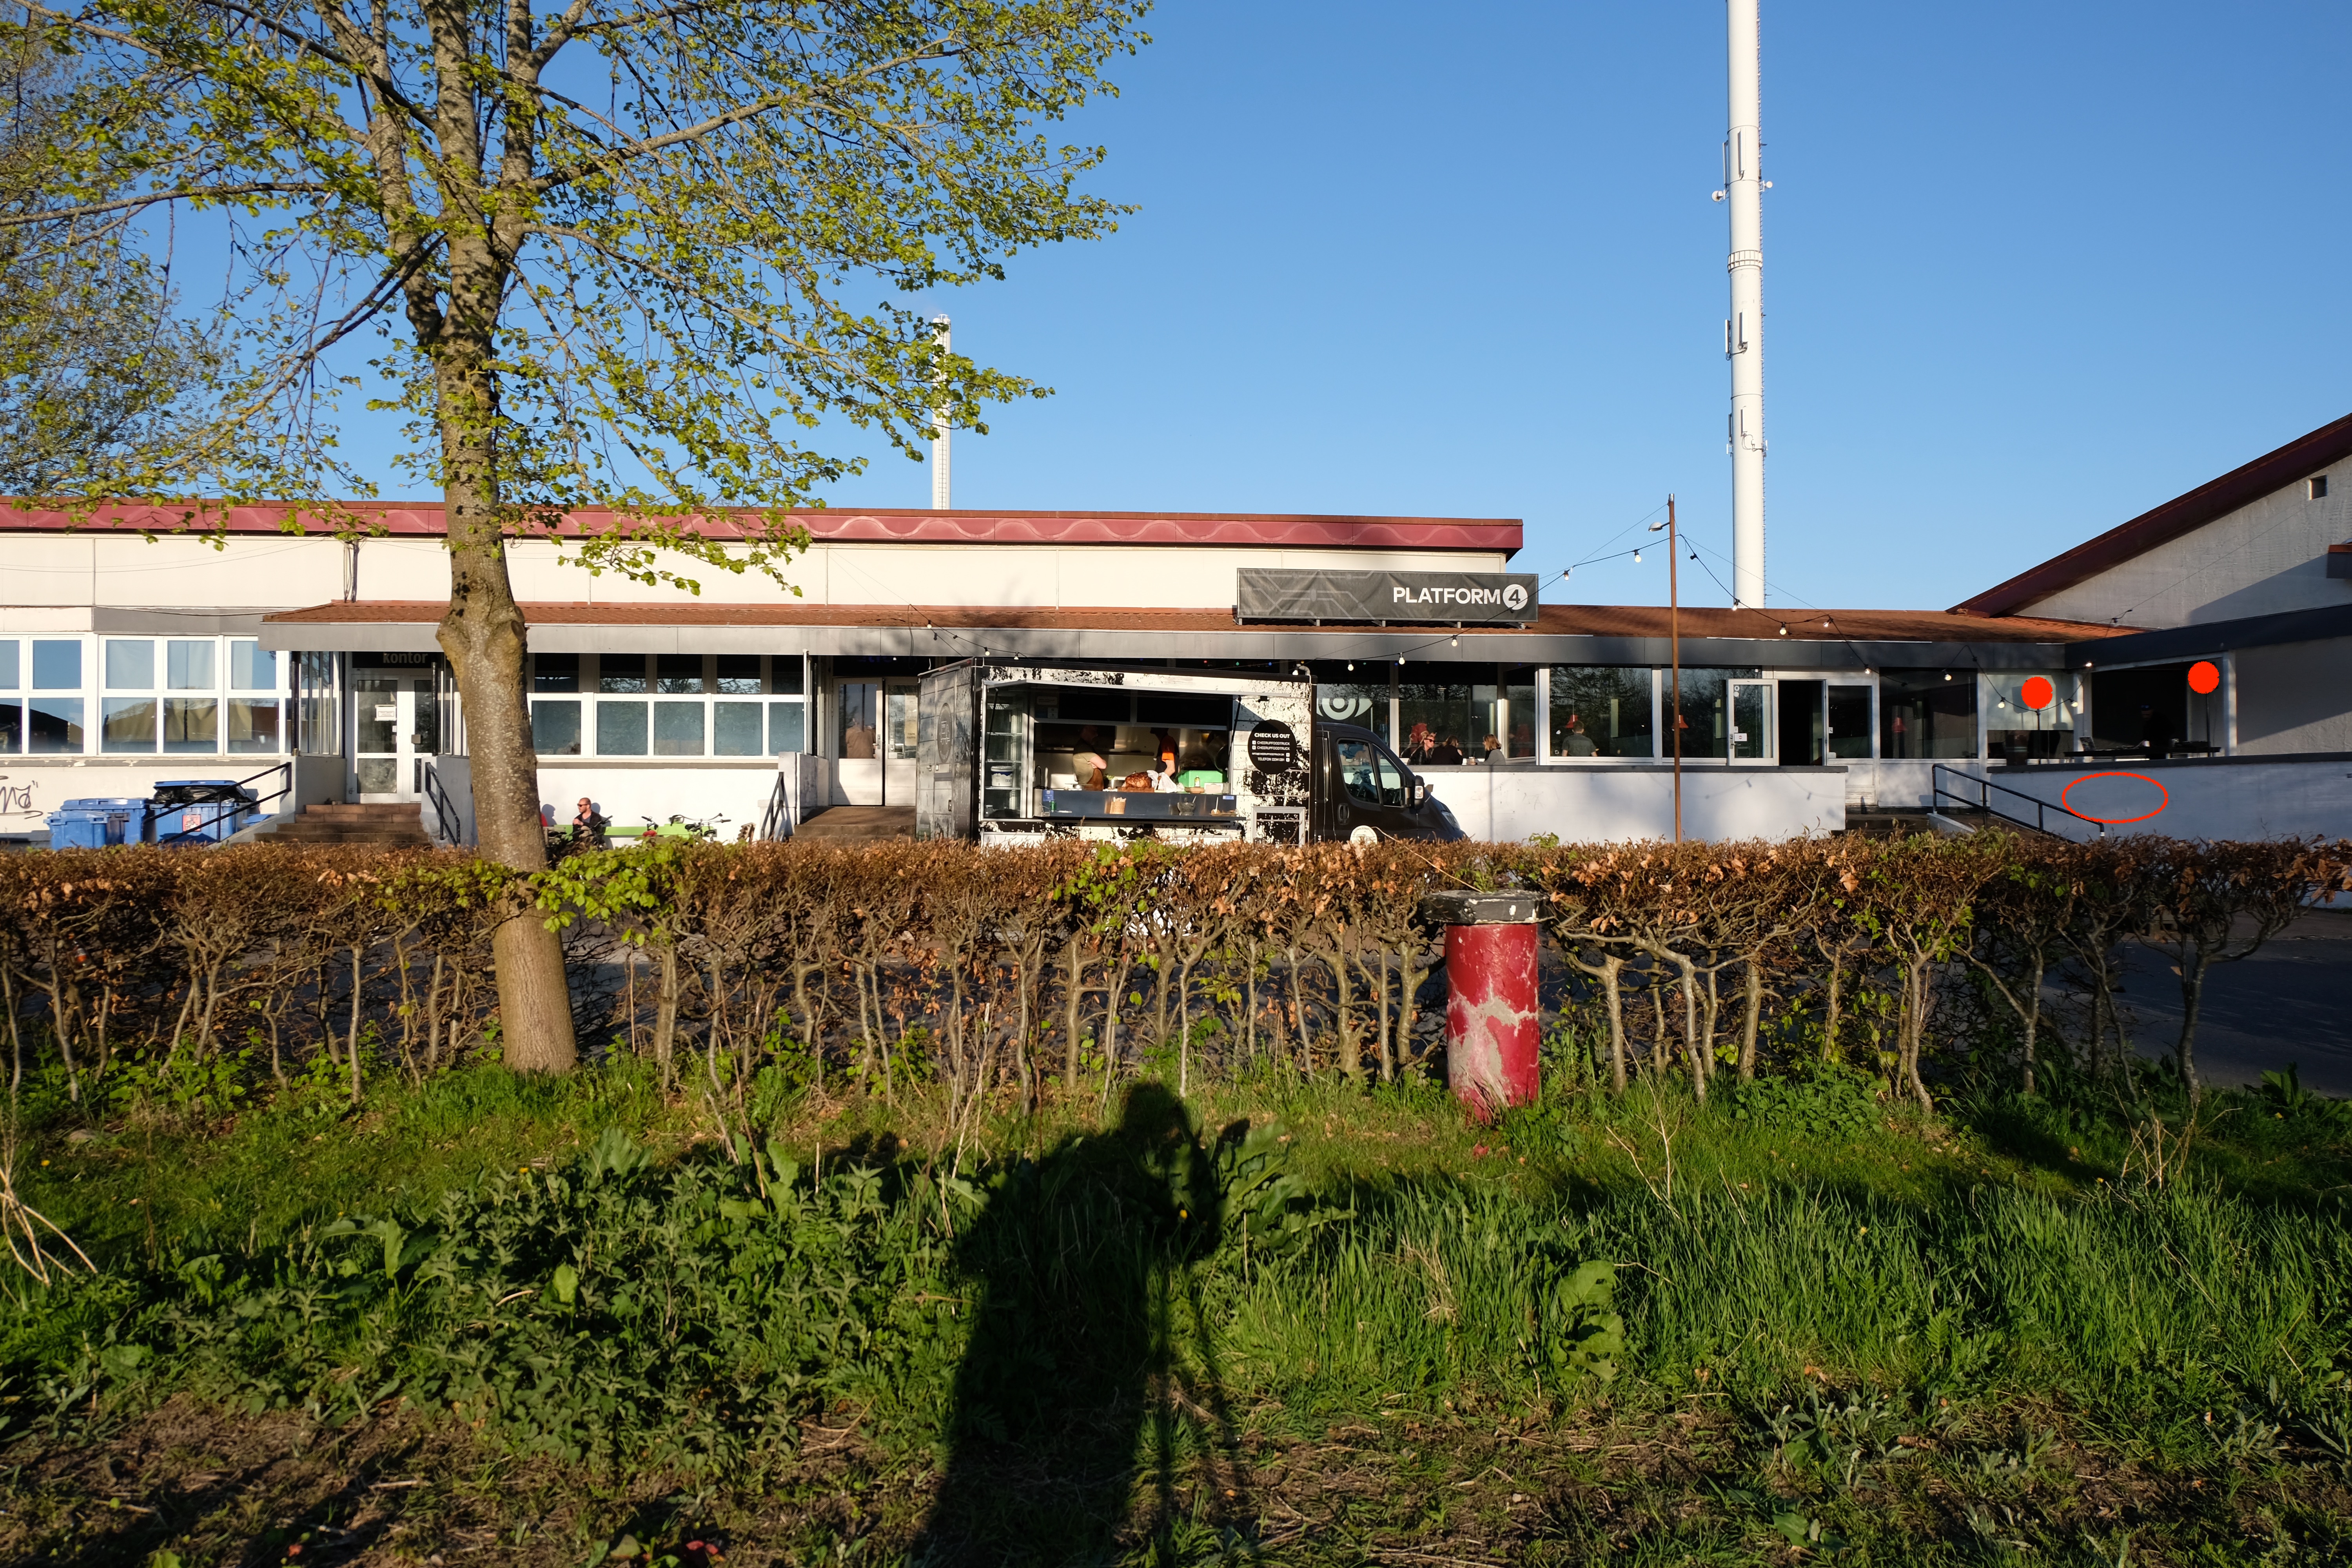
\includegraphics[width=1\textwidth]{Figures/P4day.jpg}
    \caption{picture of the setup at the center point of the microphone array}
    \label{fig:Scenario4}
\end{figure}
